\section{Implementation} \label{s:impl}
We implement the time-indexed based general ILP\footnote{We transform the ILP into its standard form and express the necessary terms as a big matrix, the details are omitted in this report but presented in the actual code.} in \S\ref{s:ilp} and a greedy list scheduling algorithm in \S\ref{s:lst}. The program takes the specification of job weights vector, processing time vector, precedence constraints 0-1 matrix (each $(i, j)$ with entry value 1 indicates $i$ precedes $j$) and number of machines as input, and outputs the weighted sum of completion time, obtained by both ILP and greedy list scheduling. The program can be used for benchmarking approximation algorithms for $P|prec|\sum w_j C_j$ in practice. The code is also open-sourced in \url{https://github.com/hongzimao/6.854/tree/master/project/code}.

We use the implementation to conduct a small scale experiment mainly for the results in \cite{schulz2011near} on the 0-1 bipartite instance. We first did a speed test on ILP approach and the greedy list approach on a 3 parallel machine scenario. The precedence constraints from a direct acyclic graph is randomly generated with the number of constraints uniformly distributed in $[n/2, n]$, where $n$ is the number of jobs. The weights and processing time are uniformly distributed in $[1, 10]$. We then extend to run 100 experiments each on an instance with number of jobs $n = [10, 15, 20, 25, 30]$. Figure \ref{fig:obj_ratio} shows the run time of the two programs averaged over the 100 experiments. As expected, we already see the trend of exponential growing run time in ILP compared with a relatively constant $O(n)$ run time of the list scheduling algorithm.

\begin{figure}[h]
	\centering
	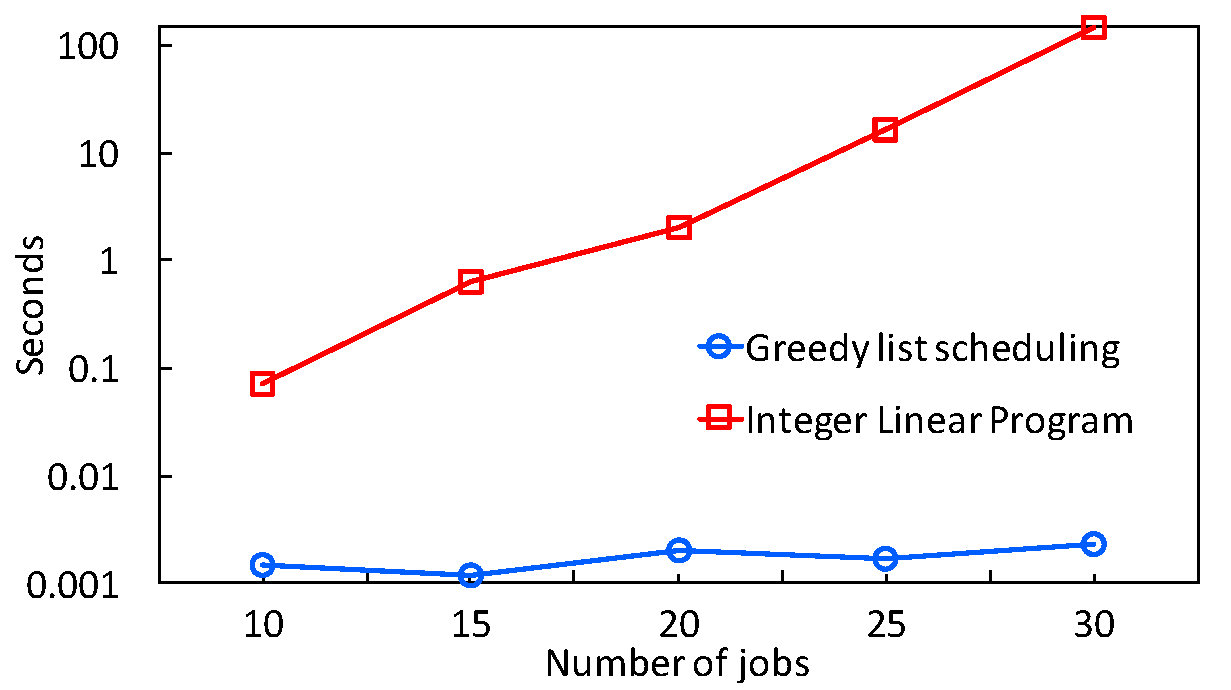
\includegraphics[width=0.6\textwidth]{figs/runtime.pdf}
	\caption{Running time comparison of ILP and simple greedy list scheduling.}
	\label{fig:runtime}
\end{figure}

Then we compare the objective ratio between the list scheduling approximation algorithm and ILP. In a general case of $P|prec|\sum w_j C_j$, as we see in the examples in \S\ref{s:lst} and \S\ref{s:lpc}, we would expect to see the objective ratio between a quickly computed feasible solution and ILP to increase as the number of job grows. In contrast, \S\ref{s:bism} shows the quality of a random solution approaching optimal as the number of job increases. In our experiment for $1|prec|\sum w_j C_j$, we accordingly fix a single machine scenario with 0-1 bipartite types of jobs. Then in 100 experiments with number of jobs $n = [10, 15, 20, 25, 30]$, we randomly assign half of the job to $N_1$ and the other half to $N_2$. For each bipartite pair in $N_1$ and $N_2$, a precedence constrain is established with $0.5$ probability, which satisfies how \S\ref{s:bism} constructs a balanced class. Then we compare the result of the objective ratio in of 3 machine general case and 0-1 bipartite instance in figure \ref{fig:obj_ratio}. The experiment matches with what we expect for the approximation bounds, where the general case has the greedy list scheduling approach progressively worse than optimal as the number of jobs grows, while 0-1 bipartite instance has the phenomenon occurs in the opposite direction. 

\begin{figure}[h]
	\centering
	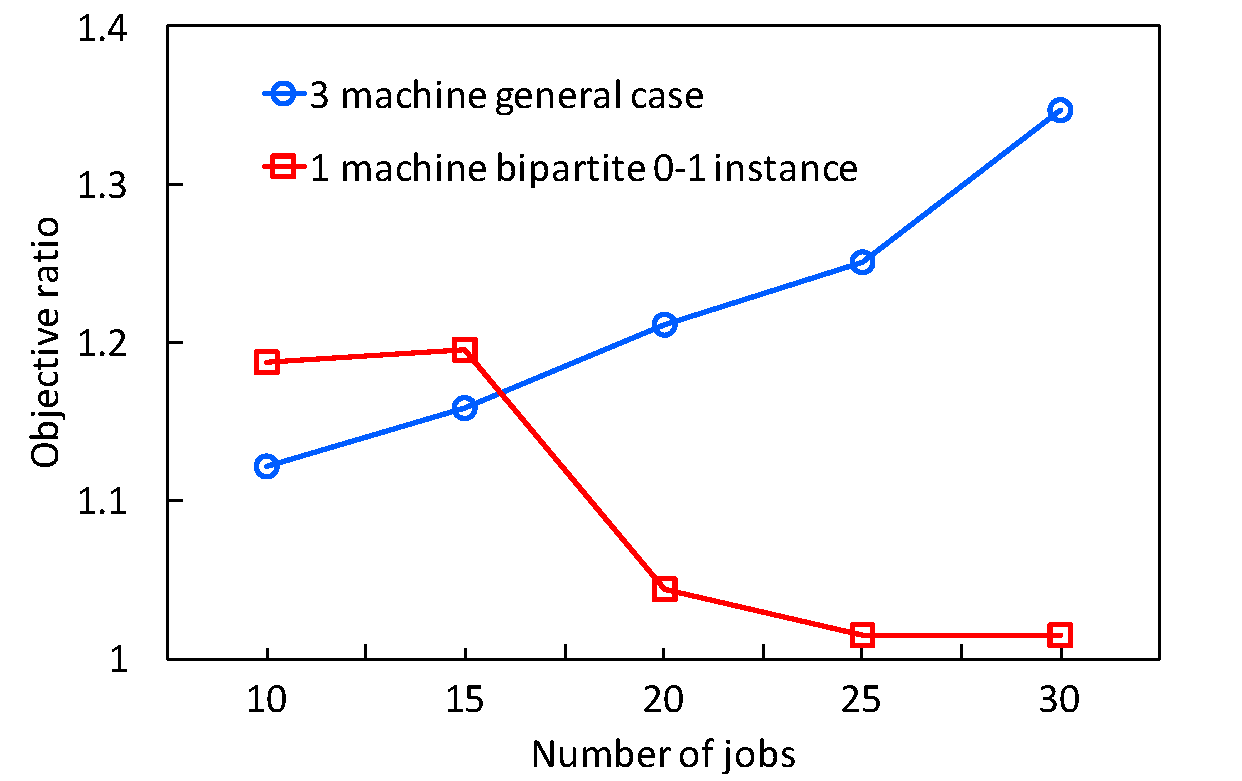
\includegraphics[width=0.6\textwidth]{figs/obj_ratio.pdf}
	\caption{Objective ratio of greedy list scheduling over ILP, on the general 3 parallel machine case and the special bipartite 0-1 instance.}
	\label{fig:obj_ratio}
\end{figure}
